%%%%%%%%%%%%%%%%%%%%%%%%%%%%%%%%%%%%%%%%%%%%%%%%%%%%%%%%%%%%%%%%%%%%%%%%%%%%%%%%
\chapter{Leistungsanalyse}
\label{sct:benchmarks}
%%%%%%%%%%%%%%%%%%%%%%%%%%%%%%%%%%%%%%%%%%%%%%%%%%%%%%%%%%%%%%%%%%%%%%%%%%%%%%%%

%%%%%%%%%%%%%%%%%%%%%%%%%%%%%%%%%%%%%%%%%%%%%%%%%%%%%%%%%%%%%%%%%%%%%%%%%%%%%%%%
\section{Rechenintensiver Testalgorithmus}
\label{sct:montecarloalgo}
%%%%%%%%%%%%%%%%%%%%%%%%%%%%%%%%%%%%%%%%%%%%%%%%%%%%%%%%%%%%%%%%%%%%%%%%%%%%%%%%

%%%%%%%%%%%%%%%%%%%%%%%%%%%%%%%%%%%%%%%%%%%%%%%%%%%%%%%%%%%%%%%%%%%%%%%%%%%%%%%%
\subsection{Monte-Carlo Algorithmen}
%%%%%%%%%%%%%%%%%%%%%%%%%%%%%%%%%%%%%%%%%%%%%%%%%%%%%%%%%%%%%%%%%%%%%%%%%%%%%%%%

Monte-Carlo-Algorithmen sind Algorithmen, die mit Hilfe von (Pseudo-)Zufallszahlen das gesuchte Ergebnis statistisch approximieren. Dafür werden Stichproben aus statistischen Verteilungen durch z.B. physkalisch begründete Abbildungen transformiert und jene Ergebnisse statistisch ausgewertet. Diese Art von Verfahren eignet sich z.B. zur Berechnung von sehr hochdimensionalen Integralen, die mit üblichen Newton-Cotes-Formeln nicht praktikabel wären. Eine andere Anwendung ist die Analyse von durch kosmischer Strahlung ausgelösten Teilchenschauern mit Hilfe von Markov-Ketten\cite{metropolis1949monte}.

Monte-Carlo-Algorithmen sind als statistische Stichprobenverfahren schon länger bekannt, wurden aber erst mit dem Aufkommen der ersten Computer, z.B. dem ENIAC um 1947-1949, praktikabel\cite{metropolis1987beginning}. Der Name, nach der Spielbank ''Monte-Carlo'', wurde von N.Metropolis vorgeschlagen und hielt sich seitdem. Der Vorschlag zu dieser Art von Algorithmus kam von John von Neumann auf, als man mit dem ENIAC thermonukleare Reaktionen simulieren wollte. Aber Fermi wird nachgesagt schon Jahre zuvor statistische Stichprobenverfahren in schaflosen Nächten händisch angewandt zu haben und mit den überraschend genauen Resultaten seine Kollegen in Staunen zu versetzen.

Monte-Carlo-Verfahren sind inhärent leicht zu parallelisieren, da eine Operation, die Simulation, mehrere Tausend oder Milliarden Mal ausgeführt wird. Eine Schwierigkeit besteht jedoch darin den Pseudozufallszahlengenerator (pseudorandom number generator - PRNG) korrekt zu parallelisieren. Das heißt vor allem muss man unabhängige Startwerte finden und an die parallelen Prozesse verteilen.
 - Zeitangaben sind hierbei nicht sinnvoll. Das betrifft alle möglichen Zeitgeber in Rechnern wie z.B. .


%%%%%%%%%%%%%%%%%%%%%%%%%%%%%%%%%%%%%%%%%%%%%%%%%%%%%%%%%%%%%%%%%%%%%%%%%%%%%%%%
\subsection{Berechnung von Pi}
%%%%%%%%%%%%%%%%%%%%%%%%%%%%%%%%%%%%%%%%%%%%%%%%%%%%%%%%%%%%%%%%%%%%%%%%%%%%%%%%

Um Pi zu berechnen wird Pi als Integral dargestellt, da sich beschränkte Integrale durch Monte-Carlo-Verfahren approximieren lassen.
\begin{equation}
	\pi = \int_\mathbb{R} \int_\mathbb{R} \begin{cases}
					1 & |x^2+y^2| \leq 1\\
					0 & \text{sonst}
			   \end{cases}
		  \mathrm{d}x\,\mathrm{d}y
\end{equation}
Das heißt wir integrieren die Fläche eines Einheitskreises. Durch die Ungleichung wissen wir auch, dass nur für $x,y\in [-1,1]$ der Integrand ungleich $0$ ist.

Da es programmatisch trivialer ist Zufallszahlen aus dem Intervall $[0,1]$ anstatt $[-1,1]$ zu ziehen, wird das Integral über den Einheitskreis in ein Integral über einen Viertelkreis geändert:
\begin{equation}
	\label{eq:piint}
	\pi = 4 \int\limits_{0}^\infty \mathrm{d}x
		    \int\limits_{0}^\infty \mathrm{d}y
		    \begin{cases}1 & |x^2+y^2| \leq 1\\0 & \text{sonst} \end{cases}
\end{equation}

%Das Vorgehen ist nun wie folgt
%\begin{enumerate}
%	\item Setze die Zählvariable \texttt{Summe} auf $0$
%	\item Ziehe für $x$ und $y$ je eine gleichverteilte Zufallszahl aus dem Intervall $[0,1]$\
%	\item Falls $x^2+y^2<1$, dann erhöhe \texttt{Summe} um $1$
%	\item Gehe zu 2.
%\end{enumerate}

Das Integral aus \autoref{eq:piint} wird nun mit
\begin{equation}
	\label{eq:pimonteint}
	\mu_N = \langle f\left( \vec{x}_i \right) \rangle := \frac{1}{N} \sum_{i=1}^N f\left( \vec{x}_i \right),\;\vec{x}_i \text{ uniform zufallsverteilt aus } \Omega:=[0,1]\times[0,1]
\end{equation}
approximiert. Im allgemein ist $f$ eine beliebige Funktion, aber für die Berechnung von Pi ist $f$ die Einheitskugel in 2D, vgl. \autoref{eq:piint}. Gemäß dem Gesetz der großen Zahlen ist dann $\lim_{N\rightarrow \infty} \mu_N = \pi$. Für den algorithmischen Ablauf siehe Algortihmus~\ref{alg:montepi}

\begin{algorithm}
    \DontPrintSemicolon
    \SetKwData{sum}{sum}
    \SetKwData{x}{x}
    \SetKwData{y}{y}
    \SetKwFunction{UniformRandom}{UniformRandom}
    \SetKwInOut{Input}{Eingabe}
    \SetKwInOut{Output}{Ausgabe}
    \Input{Anzahl an Zufallsziehungen $N$}
    \Output{Approximation von $\pi$}
    \BlankLine
    \sum$\leftarrow 0$\;
    \For{ $i\leftarrow 1$ \KwTo $N$ }{
        \x$\leftarrow$\UniformRandom{0,1}\;
        \y$\leftarrow$\UniformRandom{0,1}\;
        \If{$x^2+y^2<1$}{
            \sum$\leftarrow$\sum$+1$\;
        }
    }
    \caption{Berechnung von Trägern mittels Stichproben}
    \label{alg:montepi}
\end{algorithm}

%In Python kann man dies, wenn man sich auf Einkernprozessoren einschränkt, mit NumPy\cite{numpy} in nur wenigen zeilen niederschreiben:
%\begin{lstlisting}[language=python]
%from numpy import *
%N=10000000
%x=random.rand(N)
%y=random.rand(N)
%pi = 4.0 * sum( x*x + y*y < 1 ) / N
%\end{lstlisting}\vspace{-1.5\baselineskip}

Der Vollständigkeit halber seien kurz ein paar Worte zu den Rändern erwähnt; das betrifft die Zufallszahlen die entweder aus einem rechtsoffenem oder abgeschlossenen Intervall $[0,1]$ stammen können, d.h. der Vergleich schließt die Gleichheit mit ein oder nicht.

Aus der Integraltheorie ist klar, dass die Ränder ein Nullmaß haben und damit keine Rolle spielen. Aber für diskrete Verfahren könnte dies zu einer zusätzlichen systematischen Fehlerquelle führen, die das Fehlerskalierverhalten möglicherweise beeinträchtigt.

Am Beispiel von nur vier Zuständen für Zufallszahlen für den rechtsoffenen Fall, also $x,y\in \lbrace 0,0.25,0.5,0.75 \rbrace$, sei dies einmal durchdacht. Damit ergibt sich
\begin{equation}
	x^2+y^2 = \lbrace 0, 0.0625, 0.125, 0.25, 0.3125, 0.5, 0.5625, 0.625, 0.8125, 1.125 \rbrace
\end{equation}
% (Python-Skript für Kombinationen:
%    x=array([0,1,2,3])/4.
%    a,b=meshgrid(x**2,x**2)
%    unique( (a+b).ravel() )
Hier macht es aufgrund der begrenzten Anzahl an Zuständen, unter denen die $1.0$ ohnehin nicht auftritt, keinen Unterschied ob man $<$ oder $\leq$ vergleicht, man erhielte Pi zu $3.6$.
Hinzu kommt aber, dass Zustände auf den Grenzen $x=0$ und $y=0$ liegen, sodass die Grenzen vierfach gezählt werden da wir nur den Viertelkreis berechnen und mit vier multiplizieren.

Man hat also ohnehin immer einen Diskretisierungsfehler von $\mathcal{O}\left(\Delta x\right)$ wobei $\Delta x$ die Diskretisierungslänge zwischen zwei Zuständen ist. Angemerkt sei, dass dies für Gleitkommazahlen komplizierter gestaltet.

Abschließend sei angemerkt, dass Monte-Carlo-Methoden dafür gedacht sind einen praktisch unerschöpflichen Raum Stichprobenartig auszutesten, sodass Diskretisierungs- und Randfehler ohnehin als vernachlässigbar angenommen werden. Wenn man merkt, dass es zu Diskretisierungsfehler wie obig an den Rändern kommt, oder man gar die Anzahl aller möglichen Zustände an Zufallszahlen erschöpft hat und sich die Approximation damit nicht mehr verbessern kann, sollte man über ein anderes Verfahren nachdenken oder den Zufallsgenerator anpassen und z.B. mit 128-Bit statt 32-Bit betreiben. Auch die maximale Periodenlänge von Pseudozufallsgeneratoren spielt hier eine Rolle!
%
%Mit geschlossenen Grenzen hingegen wären $x,y\in\lbrace 0,\frac{1}{3},\frac{2}{3},1 \Rightarrow \rbrace 0, \frac{1}{9}, \frac{2}{9}, \frac{4}{9}, \frac{5}{9}, \frac{8}{9}, 1 \frac{10}{9}, \frac{13}{9},2 \rbrace$
% Man beachte, dass float ohnehin nur 32 Bit ist, wovon 1 bit das Vorzeichen und 8 bit der Exponent ist. Da wir uns immer nur im Intervall [0,1] befinden nutzen wir Vorzeichen und Exponent ohnehin nicht, sodass nur 23 Bit Präzision benutzt werden. Das sind also nur 2^23 \approx 10^7 erreichbare Zustände. Moderne Prozessoren können leicht 10^9 Operationen pro Sekunde rechnen, sodass einfache Fließkommagenauigkeit nicht ausreicht, da schon nach einigen Millionen Stichproben sich der relative Fehler nicht mehr verbessern, aber auch nciht mehr verschlechtern, wird. Siehe dazu Abb.\ref{fig:monteerrorfloat}

Da die Monte-Carlo-Pi-Integration einer Mittelwertbildung entspricht, vgl. Gl.\ref{eq:pimonteint}, ist die statistische Unsicherheit gegeben durch die Standardabweichung des Mittelwerts $\sigma_{\mu_N}$, welche gegeben ist als
\begin{equation}
	\sigma_{\mu_N} \frac{\sigma}{\sqrt{N}}
\end{equation}
wobei $\sigma$ die Standardabweichung der Stichprobe ist, vgl. Anhang~\ref{apx:meanerror}.
Wenn $f_i$ in einem beschränkten Intervall liegt, dann ist auch die Standardabweichung der Stichproben $f_i$ beschränkt, sodass die Standardabweichung auf den Mittelwert $\propto \frac{1}{\sqrt{N}}$ abnimmt.

\begin{figure}
	\centering
	\begin{minipage}{0.7\linewidth}
		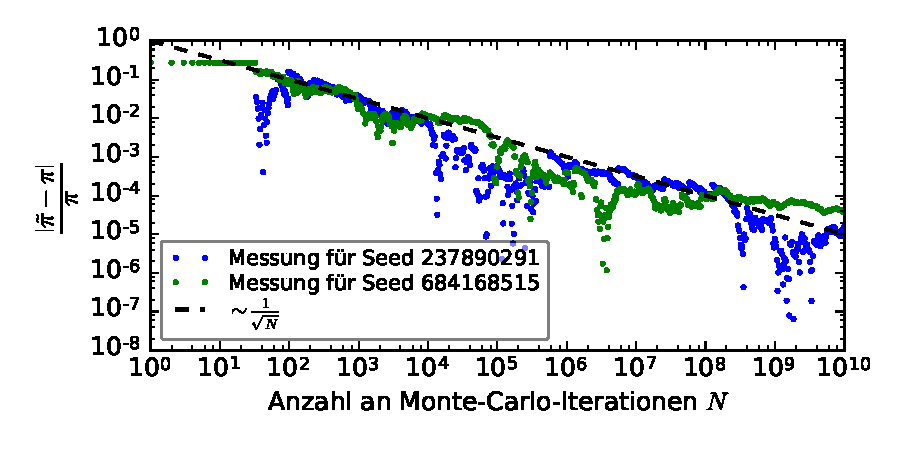
\includegraphics[width=\linewidth]{monte-carlo-pi-error-scaling}
	\end{minipage}
	\caption{captiontext}
	\label{fig:monteerrorfloat}
\end{figure}


%\subsection{Pseudozufallszahlgeneratoren}
%\section{Vergleich - Alternativen}


%%%%%%%%%%%%%%%%%%%%%%%%%%%%%%%%%%%%%%%%%%%%%%%%%%%%%%%%%%%%%%%%%%%%%%%%%%%%%%%%
\section{Testsysteme}
%%%%%%%%%%%%%%%%%%%%%%%%%%%%%%%%%%%%%%%%%%%%%%%%%%%%%%%%%%%%%%%%%%%%%%%%%%%%%%%%


%%%%%%%%%%%%%%%%%%%%%%%%%%%%%%%%%%%%%%%%%%%%%%%%%%%%%%%%%%%%%%%%%%%%%%%%%%%%%%%%
\subsection{System 1: Heimsystem}
\label{sct:system1}
%%%%%%%%%%%%%%%%%%%%%%%%%%%%%%%%%%%%%%%%%%%%%%%%%%%%%%%%%%%%%%%%%%%%%%%%%%%%%%%%


Aufgrund der leichten Verfügbarkeit und als Beispiel für Grafikkartenbeschleuniger im nicht-professionellen Verbrauchersegment, wurden einige Tests auf einem herkömmlichen Arbeitsplatzrechner ausgeführt:

\begin{table}[H]
	\begin{center}\begin{tabularx}{0.9\linewidth}{r|X}
	Prozessor & Intel(R) Core(TM) i3-3220 (Ivy-Bridge), \SI{3.30}{\giga\hertz}, 2 Kerne (4 durch SMT), AVX\cite{ark3220} \\
	Arbeitsspeicher & $4\times \SI{4}{\gibi\byte}$ DDR3 \SI{1600}{\mega\hertz} CL9\cite{corsair4gbddr3}\\
	\hline
	Grafikkarte & GigaByte GTX 760 WindForce 3X Overclocked, Codename: GK104-225-A2 (Kepler), 1152 CUDA-Kerne, \SI{1085}{\mega\hertz} ( \SI{1150}{\mega\hertz} Boost), \SI{2}{\gibi\byte} GDDR5-VRAM mit \SI{1502}{\mega\hertz} PCIe-3.0-x16-Schnittstelle\cite{gigabytegtx760,gtx760,nvidiakepler}
	\end{tabularx}\end{center}
	\caption{Heimsystemkonfiguration}
\end{table}

Die Maximalleistung in der Berechnung von Fließkommazahlen einfacher Genauigkeit (SPFLO) im Verhältnis einer Multiplikation zu einer Addition beträgt
\begin{align}
	\SI{3.30}{\giga\hertz} \cdot
	2\,\text{Kerne} \left(
		1\,\frac{ \text{AVX ADD Einheit} }{ \text{Kern} } +
		1\,\frac{ \text{AVX MUL Einheit} }{ \text{Kern} }
	\right) \cdot
	8\,\frac{ \text{SPFLO} }{ \text{AVX Einheit} } \\
	= 105.6\,\text{GSPFLOPS}
\end{align}
für den Prozessor. Informationen zur Architektur, wie die Anzahl an AVX-Einheiten wurde aus Ref.\cite{cesga} entnommen.

Die Maximalleistung der Grafikkarte beträgt:
\begin{align}
	\SI{1.085}{\giga\hertz} \cdot 1152 \text{CUDA-Kerne} \cdot
	1 \frac{ \text{FMA-Einheit} }{ \text{CUDA-Kern} } \cdot
	2 \frac{ \text{SPFLO} }{ \text{FMA-Einheit} }
	= 2500\,\text{GSPFLOPS}
\end{align}
Zugegeben, es wurde beim Prozessor gespart und bei der Grafikkarte nicht, aber der Geschwindigkeitsunterschied von 24x begründet dennoch das Interesse daran Grafikkarten zu nutzen, auch wenn es bei Grafikkarten mehr zu beachten gibt, um diese Maximalleistung erhalten zu können.



%%%%%%%%%%%%%%%%%%%%%%%%%%%%%%%%%%%%%%%%%%%%%%%%%%%%%%%%%%%%%%%%%%%%%%%%%%%%%%%%
\subsection{System 2: Taurus}
\label{sct:system2}
%%%%%%%%%%%%%%%%%%%%%%%%%%%%%%%%%%%%%%%%%%%%%%%%%%%%%%%%%%%%%%%%%%%%%%%%%%%%%%%%


Für Skalierungstests wurde einer der Hochleistungsrechner der TU-Dresden, ein Bull HPC-Cluster mit dem Namen Taurus, benutzt. Der Bau der ersten Phase von Taurus war 2013 abgeschlossen\cite{taurusnutzerschulung}. Zum Zeitpunkt der Nutzung (2015/2016) waren alle Knoten von Phase 1 schon in die 2015 fertiggestellt\cite{heisehrsk2} Phase 2 integriert wurden\cite{doctudtaurushardware} und werden nun beide unter dem Namen Taurus zusammengefasst.

\begin{figure}[H]
	\centering
	\begin{minipage}{0.5\linewidth}
		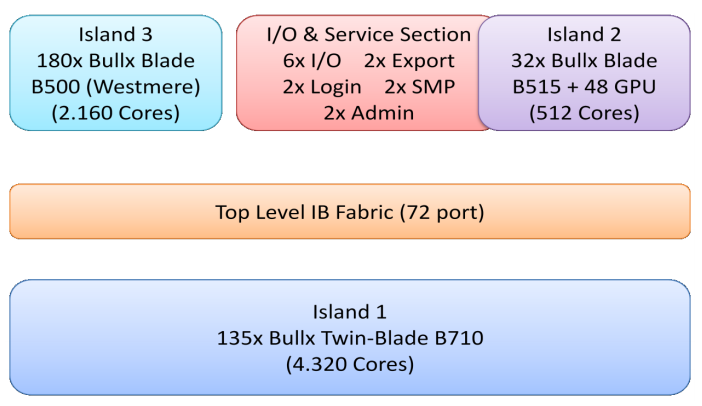
\includegraphics[width=\linewidth]{taurusphase1}
	\end{minipage}\begin{minipage}{0.5\linewidth}
		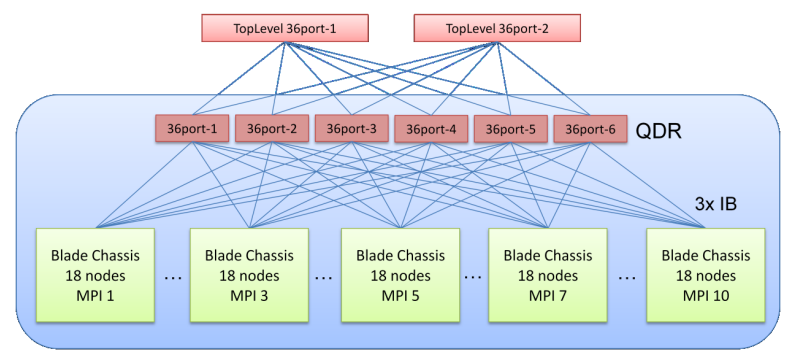
\includegraphics[width=\linewidth]{taurusphase1island1interconnects}
	\end{minipage}
	\caption{\textbf{Links:} Übersicht Taurus Phase 1. \textbf{Rechts:} Schema der Topologie von Insel 2, auf der ausschließlich gerechnet wurde. Die Bilder wurden übernommen aus Ref.\cite{taurusnutzerschulung}}
	\label{fig:taurusphase1}
\end{figure}

Gerechnet wurde auf Insel 2 von Taurus, vgl. Tabelle~\ref{tbl:island2}. Wenn nicht anders erwähnt, dann beziehen sich Benchmarks auf die Tesla K20x Knoten.

\begin{table}[H]
	\begin{tabularx}{0.9\linewidth}{r|Y|Y}
		& \textbf{Phase 1} & \textbf{Phase 2} \\
		\hline
		Knoten          & 44 & 64 \\
		Hostnamen       & taurusi2[001-044] & taurusi2[045-108] \\
		Prozessor       & 2x Intel Xeon CPU E5-2450 (8 Kerne) @ 2.10GHz, MultiThreading deaktiviert, AVX, 2x 268.8\,GSPFLOPS
						& 2x Intel(R) Xeon(R) CPU E5-2680 v3 (12 Kerne) @ 2.50GHz, MultiThreading deaktiviert, AVX2 insbesondere FMA3\cite{ark2680v3}, 2x 537.6\,GSPFLOPS \\
		GPU 			& 2x NVIDIA Tesla K20x & 4x NVIDIA Tesla K80 \\
		Arbeitsspeicher & \SI{32}{\gibi\byte} & \SI{64}{\gibi\byte} \\
		Festplatte      & \SI{128}{\gibi\byte} SSD & \SI{128}{\gibi\byte} SSD
	\end{tabularx}
	\caption{Zusammensetzung Insel 2 von Taurus\cite{doctudtaurussystem}}
	\label{tbl:island2}
\end{table}

\begin{table}[H]
	\begin{tabular}{r|c|c}
	& \textbf{K20x} & \textbf{K80} \\
	\hline
	Chip       & GK110 & GK210 \\
	Takt       & \SI{0.732}{\giga\hertz} & \SI{0.560}{\giga\hertz} \\
	CUDA-Kerne & 2688 & 4992 \\
	Speicher   & \SI{6}{\gibi\byte}, GDDR5 384 Bit Busbreite
	           & $2\times\SI{12}{\gibi\byte}$, GDDR5 384 Bit Busbreite \\
    Bandbreite & \SI{250}{\giga\byte\per\second}
	           & $2\times\SI{240}{\giga\byte\per\second}$              \\
%	\begin{minipage}{2.5cm}\begin{flushright}Theoretische\\Spitzenleistung\end{flushright}\end{minipage} & 3935\,GSPFLOPS, 1312\,GDPFLOPS
%					& 5591\,GSPFLOPS, 1864\,GDPFLOPS \\
	Theoretische    & 3935\,GSPFLOPS & 5591\,GSPFLOPS \\
	Spitzenleistung & 1312\,GDPFLOPS & 1864\,GDPFLOPS
	\end{tabular}
	\caption{Spezifikationen der Kepler-Grafikkarten von Taurus\cite{nvidiakepler,k20anandtech}}
	\label{tbl:k20k80}
\end{table}

Zu den Spitzenleistungen in Tabelle~\ref{tbl:k20k80} sei angemerkt, dass jeder CUDA-Kern einfache Fließkommagenaugigkeit berechnet und auf drei CUDA-Kerne eine Doppelpräzisionseinheit kommt, wodurch sich die DFLOPS berechnen.
Die K80 hat außerdem einen Boost-Modus mit \SI{0.875}{\giga\hertz}, also einer Leistungssteigerung von $1.56$.

\section{Monte-Carlo-Simulation verschiedener Implementationen}

In Abb.\ref{fig:montepiworkloadscaling} wurde die Ausführungszeit von Monte-Carlo-Simulationen in verschiedenen Programmiersprachen über die Anzahl an Monte-Carlo-Iterationen gemessen. Gemessen wurde die Zeit mit dem Linux \texttt{time}-Befehl und zwar die \texttt{real}-Zeit. Es fällt auf, dass alle Versionen eine Initialisierungszeit haben. Bei der C++-Version beträgt diese jedoch nur knapp \SI{30}{\milli\second}, während die reine Java-Version schon ca. \SI{70}{\milli\second} benötigt. Die Nutzung von Scala erhöht dies schon auf \SI{200}{\milli\second} und die Nutzung von Rootbeer führt eine weitere Initialisierungszeit von \SI{430}{\milli\second} ein, sodass für wenig Iterationen die Rootberversion bis zu 20x langsamer sind. Erst für 10 Milliarden Iterationen beginnt die Initialisierungszeit im Vergleich zur Rechenzeit vernachlässigbar zu werden, sodass aber da die Lastenskalierung ein lineares Verhalten annimmt. Bei der C++-Version ist dies schon bei ca. 100 Millionen Iterationen der Fall.
\begin{figure}[H]
	\centering
	\begin{minipage}{0.5\linewidth}
		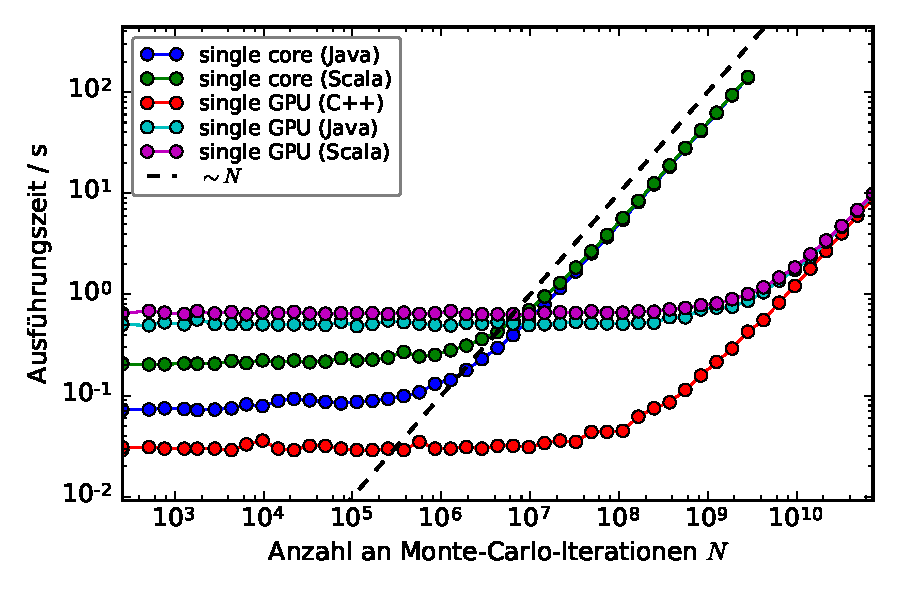
\includegraphics[width=\linewidth]{benchmarks-workload-scaling}
	\end{minipage}\begin{minipage}{0.5\linewidth}
		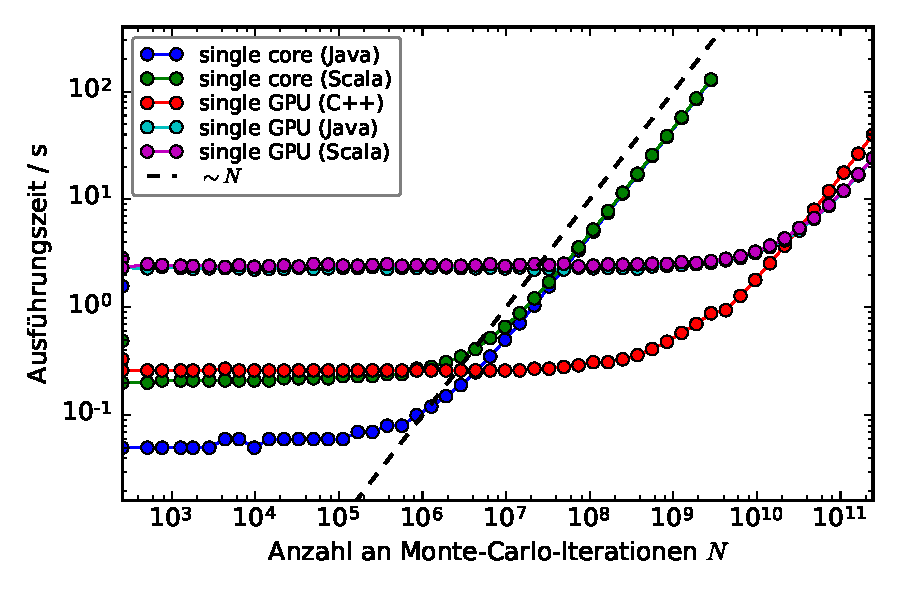
\includegraphics[width=\linewidth]{benchmarks-workload-scaling-taurus2}
	\end{minipage}
	\caption{Benötigte Ausführungszeit der Monte-Carlo Pi-Berechnung in Abhängigkeit von der Anzahl an Iterationen. Getestet auf \textbf{links:} System 1 und \textbf{rechts:} System 2 (Taurus), siehe Kapitel~\ref{sct:system1}}
	\label{fig:montepiworkloadscaling}
\end{figure}
Im Programmausdruck~\ref{lst:montemainloop} ist die Hauptschleife, die hauptsächlich die Arbeitslast generiert, zu sehen. Es handelt sich also für jede der zwei Zufallszahlen um eine Multiplikations und zwei Divisionen und dann nochmals zwei Multiplikationen für die Berechnung des Quadrat des Radius, also zusammen acht Operationen pro Iteration und neun Operationen für Iterationen die im Kreis liegen. Dies tritt für $\frac{\pi}{4}=0.785\%$ der Fälle auf, das heißt die Rechenlast, definiert als die Anzahl an arithmetischen Operationen $N_\text{Op}$ sollte sich wie folgt aus der Anzahl an Iterationen $N$ berechnen:
\begin{align}
	N_\text{Op}
	= \left[ \frac{\pi}{4}\cdot 9 + \left( 1-\frac{\pi}{4} \right)\cdot 8 \right] N
	= 8.8\cdot N
\end{align}

Zuletzt ist aus dem Plot abzulesen, dass für große Lasten wie z.B. für drei Milliarden Iterationen die Versionen, die von Grafikarten gebrauch machen, um einen Faktor $140$ (Scala) bis $320$ (C++) schneller sind als die Java Version, die auf einem Prozessor-Kern ausgeführt wird. Dieser große Unterschied zwischen CPU und GPU lässt darauf schließen, dass Java weder AVX noch mehrere Kerne gleichzeitig nutzt. Das heißt für die CPU-Versionen wäre für das Testsystem 1 noch ein Geschwindigkeitsgewinn von $8\,\frac{ \text{Op} }{ \text{AVX-Einheit} } \cdot 2\,\text{Kerne}$ erreichbar. Dies würde den Geschwindigkeitsunterschied von $320$ auf $20$ reduzieren, was in Übereinstimmung mit dem Verhältnis der Peakflops aus Kapitel~\ref{sct:system1} wäre.

\begin{lstlisting}[language=Java,caption={Hauptschleife der Monte-Carlo Pi-Berechnung},label=lst:montemainloop]
for ( int i = 0; i < dnDiceRolls; ++i )
{
    dRandomSeed = (int)( (randMagic*dRandomSeed) % randMax );
    float x = (float) dRandomSeed / randMax;
    dRandomSeed = (int)( (randMagic*dRandomSeed) % randMax );
    float y = (float) dRandomSeed / randMax;
    if ( x*x + y*y < 1.0 )
        nHits += 1;
}
\end{lstlisting}
Dieses Branching verändert also nicht das Skalierverhalten linear mit $N$, sondern führt nur zu einem veränderten Faktor. Daher ist in Abb.\ref{fig:montepiworkloadscaling} lineares Verhalten zu beobachten.



%%%%%%%%%%%%%%%%%%%%%%%%%%%%%%%%%%%%%%%%%%%%%%%%%%%%%%%%%%%%%%%%%%%%%%%%%%%%%%%%
\section{Monte-Carlo-Simulation mit Spark + Rootbeer}
%%%%%%%%%%%%%%%%%%%%%%%%%%%%%%%%%%%%%%%%%%%%%%%%%%%%%%%%%%%%%%%%%%%%%%%%%%%%%%%%


In Abbildung~\ref{fig:montepistrongscaling} ist die Laufzeit über die Anzahl an Kernen bzw. Grafikkarten dargestellt. Aus gründen der Rechenzeit wurde für eine Anzahl von $N=1,2,4,8,16,24,32$ Knoten die Leistungsanalyse für $4(N-1)$ bis $4N$ Kerne/Grafikkarten durchgeführt. Dies ist vor allem in der Abbildung rechts zu sehen, wo die Messpunkte immer in fünfer-Gruppen auftreten.

Zwar nicht in der Abbildung dargestellt, wurde auch für $4N+1$ und $4N+2$ gemessen. Das heißt Spark hat zwei mehr Slices zu verarbeiten als es Kerne gibt. Dies führt dazu, dass zwei Kerne doppelt so viel Arbeit wie der Rest haben, wodurch es zu einem sprunghaften Anstieg der Laufzeit kommt. Aus diesem Grund ist es normalerweise besser, wenn die Anzahl an Slices viel größer als die Anzahl an Kernen bzw. Grafikkarten wäre. Dies würde aber die ohnehin schon recht hohe Mindestproblemgröße noch einmal um ein, zwei weitere Größenordnungen erhöhen.

\begin{figure}[H]
	\centering
	\begin{minipage}{0.5\linewidth}
		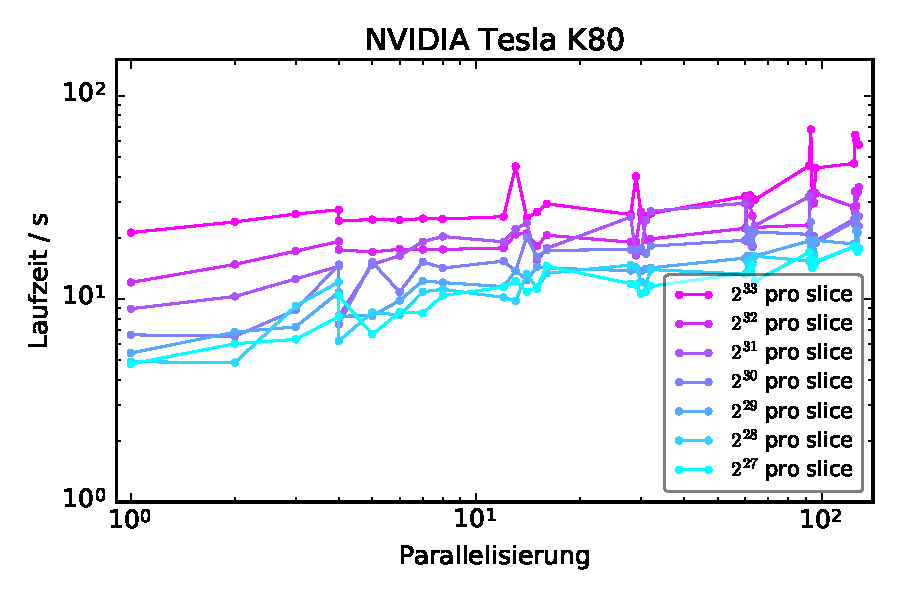
\includegraphics[width=\linewidth]{cluster-strong-scaling-gpu}
	\end{minipage}\begin{minipage}{0.5\linewidth}
		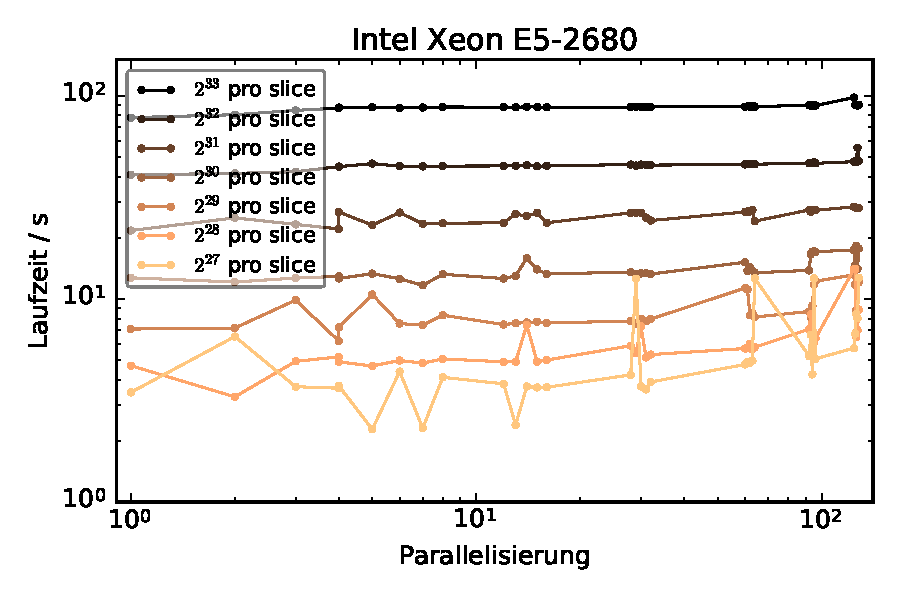
\includegraphics[width=\linewidth]{cluster-strong-scaling-cpu}
	\end{minipage}
	\caption{Benötigte Ausführungszeit der Monte-Carlo Pi-Berechnung in Abhängigkeit von der Anzahl an \textbf{links:} Kernen und \textbf{rechts:} Grafikkarten. Getestet auf System 2, siehe Kapitel~\ref{sct:system2}}
	\label{fig:montepistrongscaling}
\end{figure}

Weiterhin auffällig sind zufällig auftretende Spitzen in sowohl im CPU als auch im GPU-Benchmark. Z.b. für eine Arbeitslast von $2^33$ Iterationen pro Slice auf 24 Knoten also 92 bis 96 Grafikkarten schwankt die Ausführungszeit zwischen \SI{30}{\second}, \SI{45}{\second} und \SI{68}{\second}. Möglicherweise liegt dies an einer ungünstigen Verteilugn der Slices auf die Knoten. Die vorliegende Version nimmt eine lineare Verteilung an, sodass Slice 0 auf Grafikkarte 0 von Knoten 0 rechnet, während Slice 1 auf Grafikkarte 1 von Knoten 0 und Slice 4 auf Grafikkarte 0 von Knoten 1 rechnet. Die Zeit die eine Grafikkarte für diese Last benötigt ist \SI{22}{\second}. Es ist also wahrscheinlich, dass zumindest im Fall der \SI{68}{\second} drei verschiedene Prozesse auf einem Knoten diesselbe Grafikkarte anfordern. Diese Vermutung wurde getestet, indem jeder Slice seinen Hostnamen ausgeben soll. Mit dem Skript aus Listing~\ref{lst:start_spark_slurm.sh} ist dies schnell interaktiv getestet:
\begin{lstlisting}[language=scala]
startSpark --time=04:00:00 --nodes=5 --partition=west --gres= --cpus-per-task=12
spark-shell --master=$MASTER_ADDRESS
scala> import java.net.InetAddress
scala> sc.parallelize( 1 to 5*12, 5*12 ).map( (x) => { Thread.sleep(10); x+" : "+InetAddress.getLocalHost().getHostName() } ).collect().foreach( println )
\end{lstlisting}\vspace{-1.5\baselineskip}
Es ist also wie vermutet: die Verteilung ist nicht linear, sondern eher verzahnt, aber eigentlich zufällig.

Eine Lösung dieses Problems ist schwierig, da die Verteilung der Slices von Spark auf die Worker-Knoten opak erfolgt und es auch schwierig ist mit CUDA und vor allem mit Rootbeer herauszufinden welche der verfügbaren Grafikkarten in Benutzung ist. Ein ändern des Compute-Modus in einen Thread- oder Prozess-exklusiven Modus mittels
\begin{lstlisting}[language=bash]
nvidia-smi --compute-mode=EXCLUSIVE_PROCESS
\end{lstlisting}
ist auf Grund fehlender Berechtigungen im Cluster nicht möglich. In diesem Modus würde der Versuch eine schon in Benutzung seiende Grafikkarte anzusprechen in einer ''GPU device not available''-Fehlermeldung enden. Womöglich ist es gar nicht möglich dies über Rootbeer aus abzufangen.

Die Spitzen im CPU-Benchmark lassen sich dadurch jedoch nicht erklären, da sie für sehr Hohe Arbeitslasten kleiner verschwindet klein werden. Es handelt sich also wahrscheinlich eher um zufällige Initialisierungsoffsets oder Kommunikationslatenzen. Sie sind ungefähr \SI{3}{\second} groß, womit Kommunikationslatenz sehr unwahrscheinlich sind, da \lstinline!ping taurusi2063! als Beispiel Latenzen im Bereich von \SI{200}{\micro\second} misst. Es sei hier angemerkt, dass es in den 343 Testläufen für jeweils CPU und GPU zu zwei Fällen kam, in denen ein Job über das Spark-Web-Interface manuell beendet werden musste, da sie schon mehrere Minuten ohne Fortschritt liefen. Möglicherweise war dies aber auch ein Sympton der GPU-Konflikte pro Knoten.

In Abbildung~\ref{fig:montepistrongscaling} ist für große Arbeitslasten wie zu erwarten ein nahezu konstantes Verhalten über erhöhte Parallelisierung abzulesen. Für kleine Arbeitslasten ist eine schwache monotone Abhängigkeit zu beobachten. Möglicherweise ist dies die Zeit, die eine Reduktion über 32 Knoten länger braucht als z.B. über vier Knoten.

Die Benchmarks wurden für eine Grafikkarte pro Knoten wiederholt. Außerdem wurde leider festgestellt, dass die Benchmarks mit nur 384 Threads pro Grafikkarte ausgeführt wurden. Dies wurde geändert auf eine automatische Bestimmung, die zu ungefähr 20000 Threads führen sollte, womit Pipelining genutzt werden kann, sodass ein Faktor von 30 und mehr an Speedup zu erwarten ist.
